%This is a very basic  BE PROJECT PRELIMINARY template.

%############################################# 
%#########Author :  PROJECT###########
%#########COMPUTER ENGINEERING############


\documentclass[oneside,a4paper,12pt]{report}
%\usepackage{showframe}
%\hoffset = 8.9436619718309859154929577464789pt
%\voffset = 13.028169014084507042253521126761pt

\fancypagestyle{plain}{%
  \fancyhf{}
  \fancyfoot[CE]{Pimpri Chinchwad College of Engineering, Department of Computer Engineering 2015}
  \fancyfoot[RE]{\thepage}
}
\pagestyle{fancy}
\fancyhead{}
\renewcommand{\headrulewidth}{0pt}
\footskip = 0.625in
\cfoot{}
\rfoot{}

\usepackage{longtable}
\usepackage{float}
\usepackage{tabu}
\usepackage[]{hyperref}
\usepackage{tikz}
\usetikzlibrary{arrows,shapes,snakes,automata,backgrounds,petri}

\usepackage{tabularx}

\usepackage[nottoc,notlot,notlof,numbib]{tocbibind}
\usepackage[titletoc]{appendix}
\usepackage{titletoc}
\renewcommand{\appendixname}{Annexure}
\renewcommand{\bibname}{References}

\setcounter{secnumdepth}{5}

\usepackage{float}
\usepackage{subcaption}
\usepackage{multirow}

\usepackage[ruled,vlined]{algorithm2e}

\begin{document}

\setlength{\parindent}{0mm}
\begin{center}
{\bfseries SAVITRIBAI PHULE PUNE UNIVERSITY \\}
 \vspace*{1\baselineskip}
{\bfseries A PRELIMINARY PROJECT REPORT ON \\}
 \vspace*{2\baselineskip}
{\bfseries \fontsize{16}{12} \selectfont Hadoop add-on API for Advanced Content Based Search \& Retrieval \\ \vspace*{2\baselineskip}}
{\fontsize{12}{12} \selectfont SUBMITTED TOWARDS THE
 \\PARTIAL FULFILLMENT OF THE REQUIREMENTS OF \\

\vspace*{2\baselineskip}}
{\bfseries \fontsize{14}{12} \selectfont BACHELOR OF ENGINEERING (Computer
Engineering) \\
\vspace*{1\baselineskip}} 
%{\bfseries \fontsize{14}{12} \selectfont BY \\ 
%\vspace*{1\baselineskip}} 
%Kshama Jain  \hspace{25 mm} B120334280 \\
%Aditya Kamble  \hspace{25 mm} B120334297  \\
%Siddhesh Palande \hspace{25 mm} B120334356  \\
%Rahul Rao \hspace{25 mm} B120334381 \\
%\vspace*{2\baselineskip}
%{\bfseries \fontsize{14}{12} \selectfont Under The Guidance of \\  
%\vspace*{2\baselineskip}}
\begin{tabular}{cc}
Kshama Jain & B120334280 \\
Aditya Kamble & B120334297 \\
Siddhesh Palande & B120334356 \\
Rahul Rao & B120334381 \\[4ex]
\end{tabular}


\textbf{Under The Guidance of} \\[4ex]
Prof. Shailesh Hule \\[4ex]


\includegraphics[width=100pt]{collegelogo.jpg} \\
{\bfseries \fontsize{14}{12} \selectfont DEPARTMENT OF COMPUTER ENGINEERING \\
Pimpri Chinchwad College of Engineering \\
Sector -26, Pradhikaran, Nigdi Pune, Maharashtra 411044
}
\end{center}

\newpage



\begin{figure}[ht]
\centering

\includegraphics[width=100pt]{collegelogo.jpg}
\end{figure}


{\bfseries \fontsize{14}{12} \selectfont \centerline{Pimpri Chinchwad College of Engineering}
\centerline{DEPARTMENT OF COMPUTER ENGINEERING}
\vspace*{3\baselineskip}} 


{\bfseries \fontsize{16}{12} \selectfont \centerline{CERTIFICATE} 
\vspace*{3\baselineskip}} 

\centerline{This is to certify that the Project Entitled}
\vspace*{1\baselineskip} 


{\bfseries \fontsize{14}{12} \selectfont \centerline{Hadoop add-on API for Advanced Content Based Search \& Retrieval}
\vspace*{1\baselineskip}}

%\centerline{Submitted by}
%\vspace*{1\baselineskip} 
%\centerline{Kshama Jain  \hspace{25 mm} B120334280 } 
%\centerline{Aditya Kamble\hspace{25 mm} B120334297  } 
%\centerline{Siddhesh Palande \hspace{25 mm} B120334356 }
%\centerline{Rahul Rao \hspace{25 mm}  B120334381 }
%\vspace*{1\baselineskip} 

\begin{center}
Submitted By \\[4ex]
\begin{tabular}{cc}
Kshama Jain & B120334280 \\
Aditya Kamble & B120334297 \\
Siddhesh Palande & B120334356 \\
Rahul Rao & B120334381 \\[4ex]
\end{tabular}
\end{center}


is a bonafide work carried out by Students under the supervision of Prof. Guide Name and it
is submitted towards the partial fulfillment of the requirement of Bachelor of Engineering (Computer Engineering) Project.\\\\\\

\bgroup
\def\arraystretch{0.7}
\begin{tabular}{c c }
Prof. Shailesh Hule &  \hspace{50 mm} Prof. Dr. K. Rajeswari \\								
Internal Guide   &  \hspace{50 mm} H.O.D \\
Dept. of Computer Engg.  &	\hspace{50 mm}Dept. of Computer Engg.  \\
\end{tabular}
%}



\newpage

%\pictcertificate{TITLE OF BE PROJECT}{Student Name}{Exam Seat No}{Guide Name}
\setcounter{page}{0}
\frontmatter
\cfoot{PCCOE, Department of Computer Engineering 2015}
\rfoot{\thepage}
\pagenumbering{Roman}
%\pictack{BE PROJECT TITLE}{Guide Name}

		
{  \newpage {\bfseries \fontsize{14}{12} \selectfont \centerline{Abstract} 
\vspace*{2\baselineskip}} \setlength{\parindent}{11mm} }
{ \setlength{\parindent}{0mm} }
Unstructured data like doc, pdf, accdb is lengthy to search and filter for desired information. We need to go through every file manually for finding information. It is very time consuming and frustrating. It doesn’t need to be done this way if we can use high computing power to achieve much faster content retrieval. \\

We can use features of big data management system like Hadoop to organize unstructured data dynamically and return desired information. Hadoop provides features like Map Reduce, HDFS, HBase to filter data as per user input. Finally we can develop Hadoop Addon for content search and filtering on unstructured data. This addon will be able to provide APIs for different search results and able to download full file, part of files which are actually related to that topic. It will also provide API for context aware search results like most visited documents and much more relevant documents placed first so user work get simplified.  \\

This Addon can be used by other industries and government authorities to use Hadoop for their data retrieval as per their requirement. \\

After this addon, we are also planning to add more API features like content retrieval from scanned documents and image based documents \\


{  \newpage {\bfseries \fontsize{14}{12} \selectfont \centerline{Acknowledgments} 
\vspace*{2\baselineskip}} \setlength{\parindent}{11mm} }
{ \setlength{\parindent}{0mm} }
\textit{It gives us great pleasure in presenting the preliminary project report 
on {\bfseries \fontsize{12}{12} \selectfont Hadoop add-on API for Advanced Content Based Search \& Retrieval}.}
\vspace*{1.5\baselineskip}

 \textit{I would like to take this opportunity to thank my internal guide
 \textbf{Prof. Shailesh Hule} for giving me all the help and guidance I needed. I am
 really grateful to them for their kind support. Their valuable suggestions were very helpful.} \vspace*{1.5\baselineskip}

 \textit{I am also grateful to \textbf{Prof. Dr. K. Rajeswari}, Head of Computer
 Engineering Department, Pimpri Chinchwad College of Engineering for his indispensable
 support, suggestions.}
\vspace*{1.5\baselineskip}

\textit{In the end our special thanks to \textbf{teaching and non teaching staff} for
providing various resources such as  laboratory with all needed software platforms,
continuous Internet connection, for Our Project.}
\vspace*{3\baselineskip} \\
\begin{tabular}{p{8.2cm}c}
&Kshama Jain\\
&Aditya Kamble\\
&Siddhesh Palande\\
&Rahul Rao\\
&(B.E. Computer Engg.)
%}
\end{tabular}


% \maketitle
\tableofcontents
\listoffigures 
\listoftables



\mainmatter



  \titleformat{\chapter}[display]
{\fontsize{16}{15}\filcenter}
{\vspace*{\fill}
 \bfseries\LARGE\MakeUppercase{\chaptertitlename}~\thechapter}
{1pc}
{\bfseries\LARGE\MakeUppercase}
[\thispagestyle{empty}\vspace*{\fill}\newpage]







\setlength{\parindent}{11mm}
\chapter{Synopsis}

\section{Project Title}
Hadoop add-on API for Advanced Content Based Search \& Retrieval

\section{ Project Option }
Persistent Systems Sponsored Project

\section{Internal Guide}
Prof. Shailesh Hule 

\section{ Sponsorship and External Guide} 
Mr. Atul Shimpi ( Persistent Systems ) 


\section{Technical Keywords (As per ACM Keywords)}
\begin{itemize}
\item Hadoop
\item HDFS
\item MapReduce
\item HBase
\item Content Based System
\end{itemize}



\section{Problem Statement}
\label{sec:problem}
Hadoop add-on API for Advanced Content Based Search \& Retrieval
\section{Abstract}
Please Write here One Page Abstract. It should mainly include introduction, motivation,outcome and innovation if any.
Unstructured data like doc, pdf, accdb is lengthy to search and filter for desired information. We need to go through every file manually for finding information. It is very time consuming and frustrating. It doesn’t need to be done this way if we can use high computing power to achieve much faster content retrieval. \\

We can use features of big data management system like Hadoop to organize unstructured data dynamically and return desired information. Hadoop provides features like Map Reduce, HDFS, HBase to filter data as per user input. Finally we can develop Hadoop Addon for content search and filtering on unstructured data. This addon will be able to provide APIs for different search results and able to download full file, part of files which are actually related to that topic. It will also provide API for context aware search results like most visited documents and much more relevant documents placed first so user work get simplified.  \\

This Addon can be used by other industries and government authorities to use Hadoop for their data retrieval as per their requirement. \\

After this addon, we are also planning to add more API features like content retrieval from scanned documents and image based documents \\

\section{Goals and Objectives}
\textbf{Goals:} \\
Current Systems Focus on Search by Title,Author,etc which Is time consuming and finding relevant content from those documents is tedious task. So there is a need of such a system which shall find the relevant contents to the end user \\


\noindent \textbf{Objective:} \\
To find the relevant content from the huge number of PDF files present on Hadoop Distributed File System \\

	
\section{Relevant mathematics associated with the Project}
\noindent
S = \{s,e,x,y,DD,NDD,Mem-shared\} \\ \\
s= start state $->$ Taking input from the user as search query\\ \\ e= End State $->$ return the output to the user in the form text based content \\ \\
x = Input $->$ Search Query \\
y = Output $->$ Text Based Result \\ \\ 
DD = Deterministic Data \\
1) Number of PDF Files \\ 
2) Keyword Tokenisation and Filteration \\
3) Number of DataNodes \\
4) Search Progress \\
5) Number of Results Obtained \\ \\
NDD = Non Deterministic Data \\
1) Failure of Cluster Nodes \\
2) Communication Failure  \\ \\
Mem-Shared = Storage Space \\ 
1) HDFS will be distributed among a number of nodes in Hadoop Cluster and will share common FileSystem which will be managed by Hadoop \\



\section{Names of Conferences / Journals where papers can be published}
IFERP - International Conference Institute for Engineering Research and Publication  


\section{Review of Conference/Journal Papers supporting Project idea}
\label{sec:survey}
The reviewers committee of NIER congratulate  you for acceptance of your research paper for International Conference. You are cordially invited to convene the event by presenting your research paper through PowerPoint presentation.The Conference is being organized by NIER-India in association with "Technoarete"

\section{Plan of Project Execution}
\begin{table}[!htbp]
\begin{center}
\def\arraystretch{1.5}
  \begin{tabular}{| c | c | c | c |}
       \hline

	\textbf{Activity} & \textbf{Weeks to Spend} & \textbf{Deliverables} & \textbf{Priority}\\ \hline
	Analysis of Existing System & 2 weeks & - & Normal \\ \hline
	Requirement Gathering & 2 weeks & Requirements & Normal \\ \hline 
	Literature Survey & 3 Week & - & Normal \\ \hline
	Designing and Planning & 5 weeks & Modules & High \\ \hline
	Implementation & 10 weeks & API & High \\ \hline
	Testing & 3 weeks & Test Report & High \\ \hline
	Documentation & 4 week & Project Report & Normal \\ \hline
\end{tabular}
 \caption { Plan of Project Execution }
 \label{tab:hreq}
\end{center}

\end{table}



\chapter{Technical Keywords}
\section{Area of Project}
This  system  shall  retrieve  the  required  contents  of  files  which  are  in  an  unstructured  format containing huge amount of Data like e-books in a digital library where the number of books are present in thousands. The scope here is initially limited to PDF files which may be expanded to other unstructured formats like ePUB, mobi. \\ \\
The input is provided to the system API in the form of search query which will be firstly filtered to find the important expression as a query to the API which will return the important content to the user in the form of paragraph or text highlighted using the power of distributed computing. \\ \\
The particular page or the Entire book itself can be downloaded by the Library users if the content is satisfied else the search continues for finding relevant content

\section{Technical Keywords}
\begin{enumerate}
\item Hadoop: o Hadoop is an open-source framework that allows to store and process big data in a distributed environment across clusters of computers using simple programming models. 
\begin{itemize}
\item Distributed
\item Scalable
\item Fault-tolerant
\item Open source
\end{itemize}

\item HDFS:
\begin{itemize}
\item HDFS, the Hadoop Distributed File System, is responsible for storing data on the cluster.
\item Data is split into blocks and distributed across multiple nodes in the cluster. 
\item HDFS is a Java-based file system that provides scalable and reliable data storage, and it was designed to span large clusters of commodity servers.
\end{itemize}


\item MapReduce
\begin{itemize}
\item MapReduce is the system used to process data in the Hadoop Cluster.
\item Consist of to phases:Map and the Reduce
\item Each map task operates on discrete portion of the overall dataset
\item After all Maps are compete, the mapReduce system distributes the intermediate data to nodes which perform the Reduce phase
\end{itemize}

\item HBase
\begin{itemize}
\item HBase is an open source, non-relational, distributed database 
\item The data is partitioned based on the RowKeys into Regions.
\item Each Region contains a range of RowKeys based on their binary order.
\item A RegionServer can contain several Regions.
\end{itemize}

\item Content based:
\begin{itemize}
\item Using information manually entered or included in the table design, such as titles, descriptive keywords from a limited vocabulary, and predetermined classification schemes. The primary benefit of using content-based retrieval is reduced time and effort required to obtain image-based information.
\end{itemize}

\end{enumerate}
			
\chapter{Introduction}
\section{Project Idea}
Basic project idea is to reduce manual efforts for content based searching in large set of documents using Hadoop Big Data Management framework to automate content based searching and retrieving the relevant content. 


\section{Motivation of the Project}  
Taks like assignment completion, taking notes from text books and reference books on particular topic, topics for presentation need deep reading and need to go through every document manually just to find relevant content on given topic. \\ \\
Currently present systems are only searching based on document title, author, size, and time but not on content. So to do content based search on big data documents and large text data Haddop framework can be used. \\ \\
So using Hadoop Big Data management framework consist of HDFS, MapReduce, and HBase, we are developing content based search on PDF documents to solve real life problem. So this is basic motivation for the project. \\

\newpage

\section{Literature Survey}
{\tabulinesep=2mm
   \begin{longtabu} { |p{3.5cm} | p{3.5cm} | p{3.5cm }| p{3.5cm }|}
       \hline

\textbf{Title} & \textbf{Keyword} & \textbf{Content} & \textbf{Author}\\ \hline
Hadoop-HBase for Large- Scale  Data (2011) &
large-scale  data;  distributed  storage;  Hadoop; HDFS; Map Reduce; HBase; noSQL database &
The  paper  aims  at evaluating the performance of random reads and random writes of data storage location information to HBase and retrieving and storing  data  in  HDFS  respectively. &
Mehul Nalin Vora \\ \hline

High Performance and Fault Tolerant Distributed File System for Big Data Storage and Processing using Hadoop(2014) &
Big data; Analytics; Hadoop; Hadoop Distributed File System (HDFS); Hype cycle; MapReduce; Replication; Faulttolerance; Unstructured data &
In this paper they have highlighted the evolution and rise of big data  and discussed how HDFS produces multiple replicas of data. &
E.Sivaraman, Dr.R.Manickachezian \\ \hline

Handling Big Data Efficiently by using Map Reduce Technique(2014) &
Data Mining; Clustering; DBMS; Parallel processing; Hadoop; MapReduce. &
 In this paper, They discussed work around MapReduce, its advantages, disadvantages and how it can be used in integration with other technology. &
Seema Maitrey, C.K. Jha \\ \hline

The Dawn of Big Data - Hbase &
HBase, Hadoop Distributed File System (HDFS), HBase column oriented table. &
This paper includes the step by step introduction to the HBase,IdentifY differences between apache HBase and a traditional RDBMS. &
Vijayalakshmi Bhupathirajul, Ravi Prasad Ravud \\ \hline
      
   \end{longtabu}
}


\chapter{Problem Definition and scope}
\section{Problem Statement}
Hadoop add-on API for Advanced Content Based Search \& Retrieval

\subsection{Goals and objectives}  
\noindent \textbf{Goals:} \\
Current Systems Focus on Search by Title,Author,etc which Is time consuming and finding relevant content from those documents is tedious task. So there is a need of such a system which shall find the relevant contents to the end user \\

\noindent \textbf{Objective:} \\
To find the relevant content from the huge number of PDF files present on Hadoop Distributed File System \\


 \subsection{Statement of scope} 
This system shall retrieve the required contents of files which are in an unstructured format containing huge amount of Data like e-books in a digital library where the number of books are present in thousands. The scope here is initially limited to PDF files which may be expanded to other unstructured formats like ePUB, mobi.  \\ \\
The input is provided to the system API in the form of search query which will be firstly filtered to find the important expression as a query to the API which will return the important content to the user in the form of paragraph or text highlighted using the power of distributed computing. \\ \\
The particular page or the Entire book itself can be downloaded by the Library users if the content is satisfied else the search continues for finding relevant content 

\section{Software context} 
The end product of this project is the API for the distributed system having hadoop distributed system which would have enhanced abilities in searching the relevant contents inside big data of documents in a very rapid manner by completely harnessing the power of distributed computing and searching algorithms.This API shall be provided as an AddOn feature on top of Hadoop specially for content based retrieval purposes which would mainly deal with unstructured big data like PDF files.

\section{Major Constraints}
\begin{enumerate}
\item The first constraint is the that API used on a standalone system would not provide good performance required for content based retrieval system developed by the developer.
\item A pseudo distributed system deployed using different number of virtual machines would almost provide the similar performance as that of standalone systems depending on the number of virtual machine instances running simultaneously and the amount of memory allocated to each instance.Here care must be taken that guest nodes should not become a bottleneck to the hosted master node.
\item The best and suggested recomendation is that the API should be used and deployed on a fully-distributed system of nodes each connected to each other having independent memory ,disk and processor which will perform the best and provide expected results.
\end{enumerate}

\section{Methodologies of Problem solving and efficiency issues}
\begin{enumerate}
\item Single Mode
When a cluster with only a single node is used for implementing the content based retrieval system,slower performance is expected due to the less amount of memory and processing power.

\item Pseudo Distributed Mode
When a system is implemented either with number of virtual machines the different daemons as different process then the system is expected to perform better 

\item Fully Distributed Mode
When a cluster has number of physical nodes and hadoop daemons as different java processes with greater than 10 or more nodes in a single rack then the expected results are expected to be more better due to the presence of large storage and processing power.
\end{enumerate}

\section{Scenario in which multi-core, Embedded and Distributed Computing used}
The trends are nowadays shifting from standalone single node applications to distributed applications where in Java Frameworks like Hadoop help the applications to utlize the power of distributed computing wherein each and every node is assigned a task and the result is obtained to the master node which assigns the tasks to the slave nodes.


\section{Outcome}
\begin{enumerate}
\item The system is expected to provide the content based on the keywords entered in the form of keywords and the output shall be in the form of any of the following formats:
\item Entire Document
\item Content and the required paragraphs surrounding it
\item Only Paragraph itself 
\item Only Particular Page itself
and many such options shall be provided in the API.
\end{enumerate}

\section{Applications}
\begin{itemize}
\item Content based search and retrieval on
\begin{enumerate}
\item Digital library books 
\item IEEE Papers
\item Private Authorities
\item Government Authorities
\item Unstructured text files
\end{enumerate}

\item This API can be used to develop above functionality on platforms like
\begin{enumerate}
\item Web Application
\item Android Application
\item Standalone Application
\item Command Line Interface Application
\end{enumerate}

\end{itemize}

\section{Hardware Resources Required}
\begin{itemize}	
\item Memory require for Hadoop installation and HBase and Map Reduce components.
\item API requires minimum 100 MB space as it contains core components for content based retrieval
\item 4 GB Primary Memory / RAM
\item Intel i3/i5/i7 64bit or AMD Processors
\item SSH Authentication to communicate with Namenode and Datanodes
\end{itemize}


\section{Software Resources Required}
\begin{itemize}
\item Any Open Source Linux Distribution.(Ubuntu Server version 14.04.2 Preferred)
\item OPENSSH installed on each machine with public key of each node in authorized\_keys directory along with the localhost.
\item JDK Version 1.7 or above
\item JAVA\_HOME to be appended in the \$PATH environment variable
\item Hostname to be initialized for each node in the /etc/hosts file having a masternode (namenode), secondary namenode and various slave nodes to be added.
\item \$HADOOP\_HOME environment variable path to added in the ~/.bashrc 
\item Following Files to be configured in \$HADOOP\_HOME/etc/hadoop directory
\end{itemize}




\chapter{Project Plan}

\section{Project Estimates}
             
\subsection{Reconciled Estimates}
Reconciliation is the method of bringing together all of the data and analyses into one final estimate of value. Hence following is the total data which we have reconciled and given approx metric of all the factors. \\

\subsubsection{Cost Estimate}
The cost of project includes both hardware and software. \\[4ex]
\textbf{Hardware:} \\ \\
The total hardware cost includes the price of systems with following configuration: \\
\begin{itemize}
\item Intel Core i3 processor
\item 4 GB RAM
\item 200 GB of Hard Disk
\item NIC Card
\item Ethernet Cable
\item Wireless Router  \\
\end{itemize} 

So , the total cost will be around Rs. 80,000/- \\

\noindent \textbf{Software:} \\ \\
There is no software cost as such as all the software used for this project is open
source.


\subsubsection{Time Estimates}
The total time required is 3 months for developing the Hadoop API.


\subsection{Project Resources}
\textbf{ \\ Hardware Resources}
\begin{itemize}
\item There shall be N number of nodes each having the following hardware configuration in a fully distributed system connected environment together in a wired manner using Ethernet interface.
\item Intel i3/i5/i7 processor
\item Ethernet Interface on NIC
\item Virtualization of upto 2 or 3 nodes on a single machine for testing purposes
\item 2 or 4 GB RAM (and upto 512 MB for each node for pseudo disrtibuted) \\
\end{itemize}

\noindent \textbf{Software Resources}
\begin{itemize}
\item Any Open Source Linux Distribution.(Ubuntu Server version 14.04.2 Preferred)
\item OPENSSH installed on each machine with public key of each node in authorized\_keys directory along with the localhost.
\item JDK Version 1.7 or above
\item JAVA\_HOME to be appended in the \$PATH environment variable
\item Hostname to be initialized for each node in the /etc/hosts file having a masternode (namenode), secondary namenode and various slave nodes to be added.
\item \$HADOOP\_HOME environment variable path to added in the ~/.bashrc 
\item Following Files to be configured in \$HADOOP\_HOME/etc/hadoop directory

	\begin{enumerate}
	\item core-site.xml
	\item hadoop-env.sh
	\item yarn-site.xml
	\item mapred-site.xml
	\item master
	\item slave
	\end{enumerate}

\item Master node with Ubuntu Workstation version preferred for supporting Eclipse IDE with Hadoop plugin for development and Server having Ubuntu Server version Preferred. \\
\end{itemize}

\noindent \textbf{Tools}
\begin{itemize}
\item Eclipse IDE
\item Hadoop Eclipse Plugin
\item Java 1.7
\item Hadoop Java Libraries.
\end{itemize}

\section{Project Schedule}  
\subsection{Project task set}  
Major Tasks in the Project stages are: 
\begin{itemize}
\item Create distributed system with Hadoop namenodes and datanodes
\item Develop API methods for extracting keywords from input query
\item Test API methods for finding keywords from input query
\item Develop API methods to perform keyword search on HDFS data using Map Reduce operations
\item Test API methods to perform keyword search on HDFS data using Map Reduce operations
\item Design database schema for indexing each and every document in HDFS
\item Schema validation for HBase indexing database
\item Develop background service for indexing newly added data to HBase database automatically
\item Test background service for indexing newly added data to HBase database is working automatically or not
\item Integrating all modules
\item Integration testing
\end{itemize}

\subsection{Task network}  
\begin{center}
	\begin{figure}[!htbp]
		\centering
		\fbox{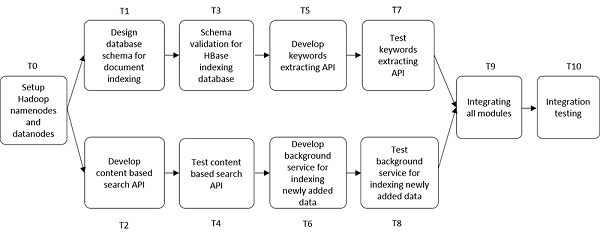
\includegraphics[width=\textwidth]{task_network}}
	  \caption{Task network}
	  \label{fig:usecase}
	\end{figure}
\end{center}  

\subsection{Timeline Chart}  
\begin{center}
	\begin{figure}[!htbp]
		\centering
		\fbox{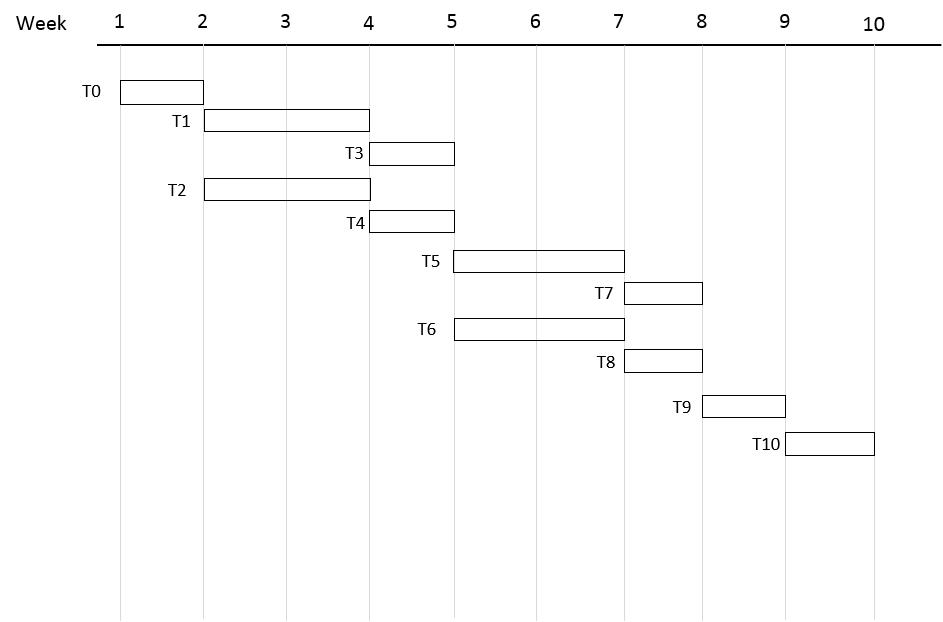
\includegraphics[width=\textwidth]{timeline_chart}}
	  \caption{Timeline Chart}
	  \label{fig:usecase}
	\end{figure}
\end{center}  
 
\section{Team Organization}
For this project team is of 4 developers. 
\begin{table}[!htbp]
\begin{center}
\def\arraystretch{1.5}
  \begin{tabular}{| c | c |}
       \hline
       
Team Member & Roles \\ \hline
Kshama Jain & Literature Survey and Solution Analysis \\ \hline
Aditya Kamble & Software API Development and Testing \\ \hline
Rahul Rao & System Management and API Development \\ \hline
Siddhesh Palande & Integration and Testing \\ \hline
       
\end{tabular}
 \caption { Team Structure }
 \label{tab:hreq}
\end{center}

\end{table}


\subsection{Team structure}
The team structure for the project is of 4 people . Roles are defined as mentioned above

\subsection{Management reporting and communication}
The communication and reporting of work is done on weekly basis depending upon the time which is around 4hrs for a week and since they are sharing the same premises the communication is also excellent
 
\chapter{Software requirement specification  (SRS is to be prepared using relevant mathematics derived and software engg. Indicators in Annex A and B)}

\section{Introduction}
\subsection{Purpose and Scope of Document}
This system shall retrieve the required contents of files which are in an unstructured format containing huge amount of Data like e-books in a digital library where the number of books are present in thousands. The scope here is initially limited to PDF files which may be expanded to other unstructured formats like ePUB, mobi. \\ \\
The input is provided to the system API in the form of search query which will be firstly filtered to find the important expression as a query to the API which will return the important content to the user in the form of paragraph or text highlighted using the power of distributed computing. \\ \\
The particular page or the Entire book itself can be downloaded by the Library users if the content is satisfied else the search continues for finding relevant content.

\subsection{Overview of responsibilities of Developer}
\begin{enumerate}
\item The developer should have the knowledge of Hadoop.
\item The developer should have the knowledge of Mapreduce and HBase.
\item The developer should have the knowledge of Java.
\end{enumerate}


  
\section{Usage Scenario}
This section provides various usage scenarios for the system to be developed.  
 \subsection{User profiles}  
There will be number of users who will use the same application which will be provided by the developer. As the user search for query in the HDFS of Distributed Hadoop System, system will return the result with expected outcome. 

\subsection{Use-cases}
All use-cases for the software are presented.

\begin{table}[!htbp]
\begin{center}
%\def\arraystretch{1.5}
\def\arraystretch{1.5}
\begin{tabularx}{\textwidth}{| c | c | c | c | X |}
\hline
Sr No.	& Use Case	& Description	& Actors	& Assumptions \\
\hline
1 & Use case 1 & User & Add Document & User add document to HDFS system using API  Insert user added document to HDFS and scan for keywords to store in metadata.
\\ \hline
2 & Use case 2 & Administrator & Setup Hadoop cluster. & Hadoop cluster will work with our addon API for content based retrieval. \\ \hline

\hline
\end{tabularx}
\end{center}
\caption{Use Cases}
\label{tab:usecase}
\end{table}


\subsection{Use Case View}
Use Case Diagram. Example is given below
\begin{center}
	\begin{figure}[H]
		\centering
		\fbox{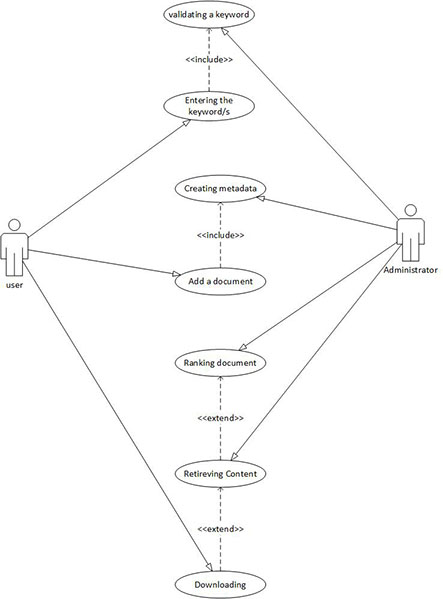
\includegraphics[width=\textwidth]{use_case_diagram}}
	  \caption{Use case diagram}
	  \label{fig:usecase}
	\end{figure}
\end{center}  

\section{Data Model and Description}  
\subsection{Data Description}  
In this project we are searching and retrieving information from data inside HDFS. Hadoop Map Reduce operations will be used to perform key value pair generation and depend upon result information is searched. \\ \\
Here, data is documents in PDF ( Portable Document Format ) format. These documents are stored on HDFS - Hadoop Distributed File System. These documents are considered as raw data. These documents can have properties like 
\begin{itemize}
\item Name
\item Size
\item Date
\item Author 
\end{itemize}
Document meta data is also maintain in HBase distributed database. It has attributes like
\begin{itemize}
\item Content Keywords
\item Index Keyword
\item Document Keywords
\end{itemize}
This information will be useful to filter documents before performing content based  searching operations.


\subsection{Data objects and Relationships}
Use Case Diagram. Example is given below
\begin{center}
	\begin{figure}[H]
		\centering
		\fbox{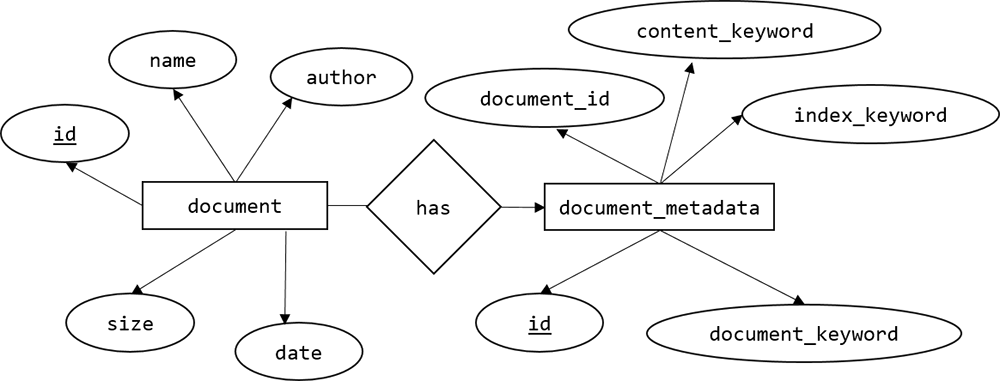
\includegraphics[width=\textwidth]{data_model}}
	  \caption{Data Model}
	  \label{fig:usecase}
	\end{figure}
\end{center}  
 
 
\section{Functional Model and Description}  
A description of each major software function, along with data flow (structured analysis) or class hierarchy (Analysis Class diagram with class description for object oriented system) is presented. 
\subsection{Data Flow Diagram}  
Use Case Diagram. Example is given below
\begin{center}
	\begin{figure}[H]
		\centering
		\fbox{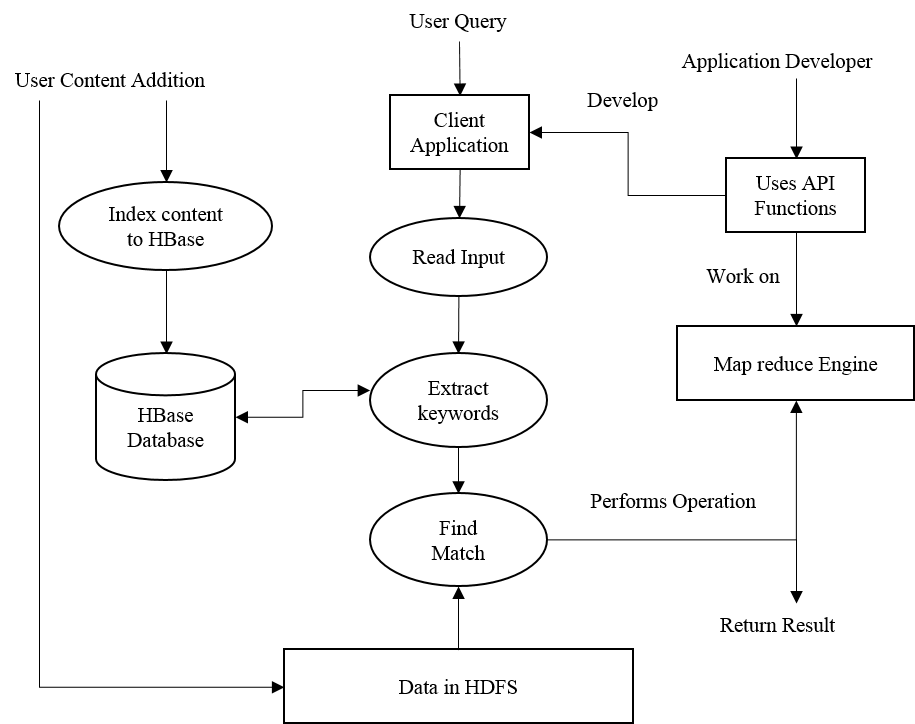
\includegraphics[width=\textwidth]{data_flow}}
	  \caption{Data Flow Diagram}
	  \label{fig:usecase}
	\end{figure}
\end{center} 
 
\subsection{Description of functions}  
A description of each software function is presented. A processing narrative for function n is presented
 
\subsection{Activity Diagram:}
\begin{center}
	\begin{figure}[H]
		\centering
		\fbox{
\includegraphics[height=430pt]{activity_diagram}}
	  \caption{Activity diagram}
	  \label{fig:act-dig}
	\end{figure}
\end{center}  

\subsection{Non Functional Requirements:}
\textbf{Performance Requirements} \\ \\
Memory Requirements:
\begin{itemize}	
\item Memory require for Hadoop installation and HBase and Map Reduce components.
\item API requires minimum 100 MB space as it contains core components for content based retrieval
\item 4 GB Primary Memory / RAM
\end{itemize}

Speed Requirements:
\begin{itemize}
\item Intel i3/i5/i7 64bit or AMD Processors
\end{itemize}

\textbf{Security Requirements}
\begin{itemize}
\item SSH Authentication to communicate with Namenode and Datanodes
\end{itemize}

\textbf{Software Quality Attributes}

Software Quality can be defined as “the conformance to explicitly stated functional and performance requirements, explicitly documented development standards, and implicit characteristics that are expected of all professionally developed software”.\\
	
\textbf{Software Quality Attributes are}

\begin{enumerate}
\item \textbf{Functionality} \\
This is an ability by which the software satisfies the needs of the software denoted by suitability, accuracy, interoperability, compliance and security.

\item \textbf{Reliability} \\
Due to wired connectivity, reliability can be guaranteed.

\item \textbf{Availability} \\
The system should be available during their respected hours.

\item \textbf{Usability} \\
This ability indicates that the usefulness of the software.

\item \textbf{Efficiency} \\
This indicates the measure of computing resources and time required by the program to perform.

\item \textbf{Maintainability} \\
The ability required to locate or fix bugs in software. There should be facility to add or delete or update documents.

\item \textbf{Portability} \\
The software works properly even if the environment gets changed (i.e. change in hardware or software).

\item \textbf{Reusability} \\
With new versions of Hadoop this API can be improved using new features of Hadoop
\end{enumerate}



\subsection{State Diagram:}	
State diagram represents the various states that an object attains during its lifecycle in response to events. A state depicts a condition of an object and the activities of an object during its lifecycle. \\
	We model the dynamic aspects of a system by using “State diagrams”. Therefore we create a state diagram for the objects that respond to events. The various constituents of a state diagram are:
\begin{itemize}
\item State machines
\item Events
\item Transitions
\end{itemize}



\begin{center}
	\begin{figure}[H]
		\centering
		\fbox{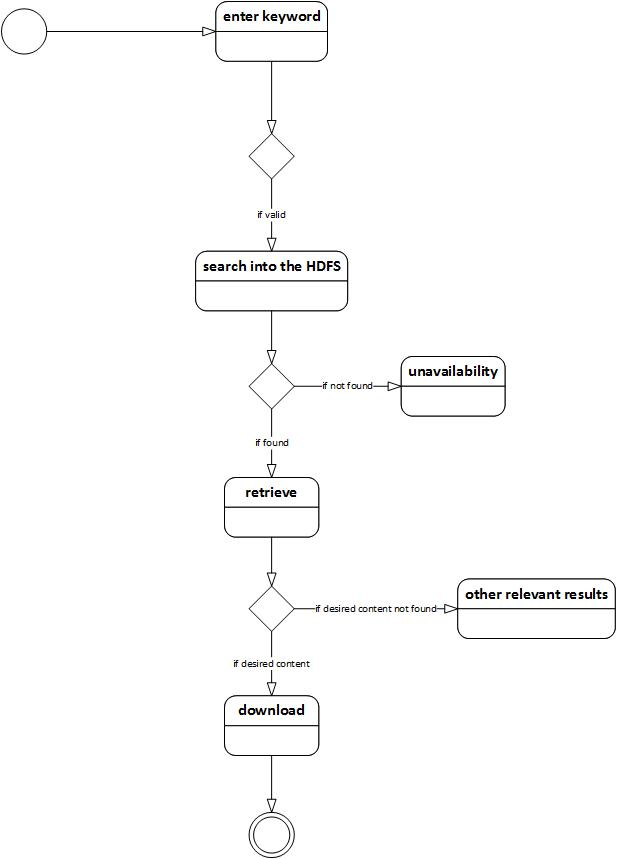
\includegraphics[width=230pt]{statemachine_diagram}}
	  \caption{State transition diagram}
	  \label{fig:state-dig}
	\end{figure}
\end{center} 
 
 \subsection{Design Constraints}	
The primary design constraint is the distributed platform. Since the application is designated for distributed systems. Creating a Application Programming  Interface which is both effective and easily usable will pose a difficult challenge. Other constraints such as limited memory and processing power are also worth considering.

 \subsection{Software Interface Description}	 
\begin{itemize}
\item Any Open Source Linux Distribution.(Ubuntu Server version 14.04.2 Preferred)
\item OPENSSH installed on each machine with public key of each node in authorized\_keys directory along with the localhost.
\item JDK Version 1.7 or above
\item JAVA\_HOME to be appended in the \$PATH environment variable
\item Hostname to be initialized for each node in the /etc/hosts file having a masternode (namenode), secondary namenode and various slave nodes to be added.
\item \$HADOOP\_HOME environment variable path to added in the ~/.bashrc 
\item Following Files to be configured in \$HADOOP\_HOME/etc/hadoop directory

	\begin{enumerate}
	\item core-site.xml
	\item hadoop-env.sh
	\item yarn-site.xml
	\item mapred-site.xml
	\item master
	\item slave
	\end{enumerate}

\item Master node with Ubuntu Workstation version preferred for supporting Eclipse IDE with Hadoop plugin for development and Server having Ubuntu Server version Preferred.
\end{itemize}



\chapter{Detailed Design Document using Appendix A and B}
 \section{Introduction}  
This document specifies the design that is used to solve the problem of Product.  

\section{Architectural Design}  
 
  \begin{center}
	\begin{figure}[!htbp]
		\centering
		\fbox{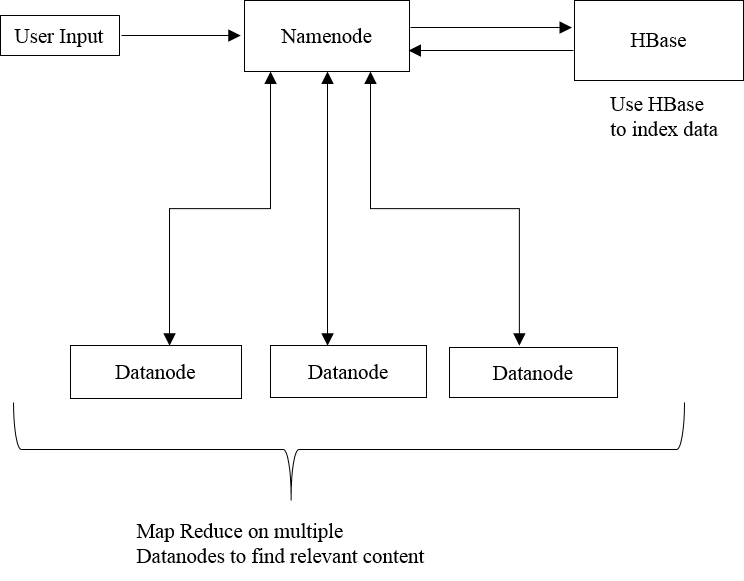
\includegraphics[width=\textwidth]{architecture_design}}
	  \caption{Architecture diagram}
	  \label{fig:arch-dig}
	\end{figure}
\end{center} 


\section{Data design (using Appendices A and B)}   

\subsection{Internal software data structure}
We are using HashMap as internal datastructure since MapReduce uses it. \\
A HashMap is an object that maps keys to values. A map cannot contain duplicate keys: Each key can map to at most one value. It models the mathematical function abstraction. The Map interface includes methods for basic operations (such as put, get, remove, containsKey, containsValue, size, and empty), bulk operations (such as putAll and clear), and collection views (such as keySet, entrySet, and values). \\
Creating Hashmap datastructure: Map<String, Integer> m = new HashMap<String, Integer>(); \\ \\
     
The second argument is a conditional expression that has the effect of setting the frequency to one if the word has never been seen before or one more than its current value if the word has already been seen. Try running this program with the command:
java Freq if it is to be it is up to me to delegate
The program yields the following output.
8 distinct words: {to=3, delegate=1, be=1, it=2, up=1, if=1, me=1, is=2}
Suppose we prefer to see the frequency table in alphabetical order. All you have to do is change the implementation type of the Map from HashMap to TreeMap. Making this four-character change causes the program to generate the following output from the same command line.
8 distinct words: {be=1, delegate=1, if=1, is=2, it=2, me=1, to=3, up=1}
Similarly, we make the program print the frequency table in the order the words first appear on the command line simply by changing the implementation type of the map to LinkedHashMap. Doing so results in the following output.
8 distinct words: {if=1, it=2, is=2, to=3, be=1, up=1, me=1, delegate=1


\subsection{Global data structure}
We are using Set interface as Global datastructure.\\
	A Set is a Collection that cannot contain duplicate elements. It models the mathematical set abstraction. The Set interface contains only methods inherited from Collection and adds the restriction that duplicate elements are prohibited. Set also adds a stronger contract on the behavior of the equals and hashCode operations, allowing Set instances to be compared meaningfully even if their implementation types differ. Two Set instances are equal if they contain the same elements.\\
The Java platform contains three general-purpose Set implementations: HashSet, TreeSet, and LinkedHashSet. HashSet, which stores its elements in a hash table, is the best-performing implementation; however it makes no guarantees concerning the order of iteration. TreeSet, which stores its elements in a red-black tree, orders its elements based on their values; it is substantially slower than HashSet. LinkedHashSet, which is implemented as a hash table with a linked list running through it, orders its elements based on the order in which they were inserted into the set (insertion-order). LinkedHashSet spares its clients from the unspecified, generally chaotic ordering provided by HashSet at a cost that is only slightly higher.


\subsection{Temporary data structure}
Arrays as temporary datastructures: \\
An array is an object of reference type which contains a fixed number of components of the same type; the length of an array is immutable. Creating an instance of an array requires knowledge of the length and component type. Each component may be a primitive type (e.g. byte, int, or double), a reference type (e.g. String, Object, or java.nio.CharBuffer), or an array. Multi-dimensional arrays are really just arrays which contain components of array type. \\
Arrays are implemented in the Java virtual machine. The only methods on arrays are those inherited from Object. The length of an array is not part of its type; arrays have a length field which is accessible via java.lang.reflect.Array.getLength().
Reflection provides methods for accessing array types and array component types, creating new arrays, and retrieving and setting array component values.


\subsection{Database description}
\begin{table}[!htbp]
\begin{center}
\def\arraystretch{1.5}
  \begin{tabular}{| c | c |}
       \hline
       
Fields & Type \\ \hline
id & int \\ \hline
name & varchar(50) \\ \hline
author & varchar(50) \\ \hline
size & int \\ \hline
date & date \\ \hline
       
\end{tabular}
 \caption { Table - Document  }
 \label{tab:hreq}
\end{center}

\end{table}

\subsection{Database description}
\begin{table}[!htbp]
\begin{center}
\def\arraystretch{1.5}
  \begin{tabular}{| c | c |}
       \hline
       
Fields & Type \\ \hline
document\_id & int \\ \hline
content\_keyword & varchar(50) \\ \hline
index\_keyword & varchar(50) \\ \hline
document\_keyword & varchar(50) \\ \hline
       
\end{tabular}
 \caption { Table - Document Metadata  }
 \label{tab:hreq}
\end{center}

\end{table}


\section{Compoent Design} 
Class diagrams, Interaction Diagrams, Algorithms. Description of each component description required.
\subsection{Class Diagram}
\begin{figure}[H]
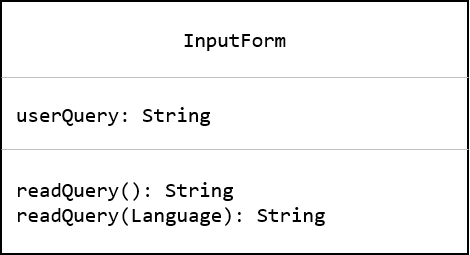
\includegraphics{class_input_form}
\end{figure}

\begin{figure}[H]
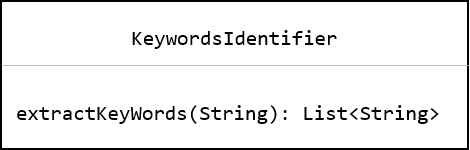
\includegraphics{class_keyword_identifier}
\end{figure}

\begin{figure}[H]
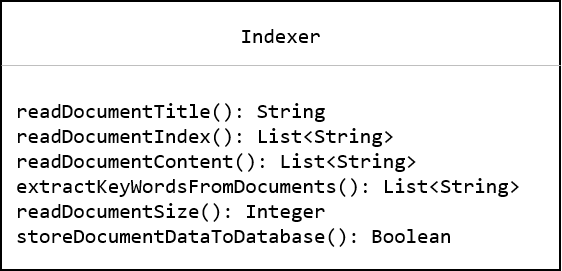
\includegraphics{class_indexer}
\end{figure}

\begin{figure}[H]
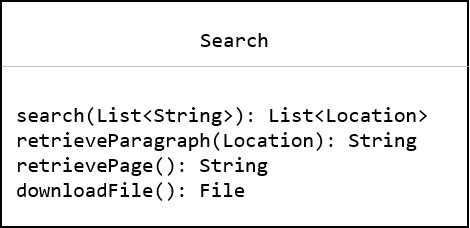
\includegraphics{class_search}
\end{figure}

\begin{figure}[H]
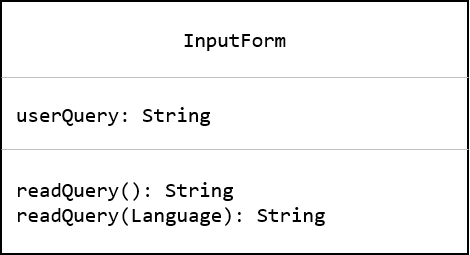
\includegraphics{class_input_form}
\end{figure}

\begin{figure}[H]
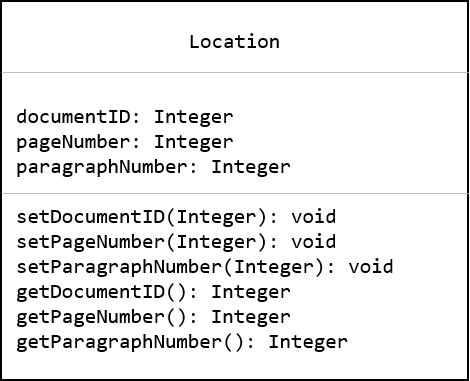
\includegraphics{class_location}
\end{figure}

 
 \chapter{Summary and Conclusion}
\section{Summery}
Unstructured data like doc, pdf, accdb is lengthy to search and filter for desired information. We need to go through every file manually for finding information. It is very time consuming and frustrating. It doesn’t need to be done this way if we can use high computing power to achieve much faster content retrieval. This addon will be able to provide APIs for different search results and able to download full file, part of files which are actually related to that topic. It will also provide API for context aware search results like most visited documents and much more relevant documents placed first so user work get simplified.    

\section{Conclusion}
Thus we can use this API in Hadoop to reduce manual efforts and bring advance content based search and retrieval

\begin{thebibliography}{7}
\bibitem {R1} Lars George, "HBase: The Definitive Guide", 1st edition, O'Reilly Media, September 2011, ISBN 9781449396107


\bibitem {R2} Tom White, "Hadoop: The Definitive Guide", 1st edition, O'Reilly Media, June 2009, ISBN 9780596521974

\bibitem {R3} Apache  Hadoop HDFS homepage http://hadoop.apache.org/hdfs/

\bibitem {R4} Mehul Nalin Vora ,"Hadoop-HBase for Large-Scale Data",Innovation Labs,PERC,ICCNT Conference

\bibitem {R5} Yijun Bei,Zhen Lin,Chen Zhao,Xiaojun Zhu ,"HBase System-based Distributed Framework for Searching Large Graph Databases",ICCNT Conference


\bibitem {R6} Seema Maitrey,C.K."Handling Big Data Efficiently by using Map Reduce Technique",ICCICT

\bibitem {R7} Maitrey S, Jha. An Integrated Approach for CURE Clustering using Map-Reduce Technique. In Proceedings of Elsevier,ISBN 978-81- 910691-6-3,2 nd August 2013.


\end{thebibliography}


\begin{appendices}

% \chapter{ALGORITHMIC DESIGN}
\chapter{Laboratory assignments on Project Analysis of Algorithmic Design}
To develop the problem under consideration and justify feasibilty using concepts of knowledge canvas and IDEA Matrix.

  \begin{center}
	\begin{figure}[!htbp]
		\centering
		\fbox{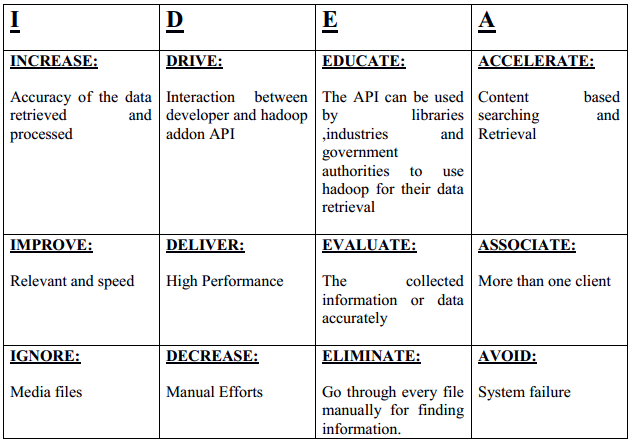
\includegraphics[width=\textwidth]{idea_matrix}}
	  \caption{IDEA Matrix}
	  \label{fig:arch-dig}
	\end{figure}
\end{center} 

\noindent  \textbf{Project problem statement feasibility assessment using NP Hard   NP complete or satisfiability issues  using modern algebra and/or relevant mathematical models.} \\

\noindent \textbf{Input:}  A set of input keywords taken as a search query  \\ 
\noindent \textbf{Output:} Question: Whether given recommendation is satisfiable or not? \\ \\

\noindent \textbf{P Class Problem : } \\
Since the Application Programming Interface has a searching algorithm which works on map-reduce engine to retrieve the content from HDFS and return the result in the form of paragraph and with relevant contents with the link to download whole document or only a part of it. \\ \\

\noindent \textbf{NP Class :} \\
The problem gets converted into NP Class when there is a verifier process to verify the content retrieved by the API . \\


\chapter{Laboratory assignments on Project Quality and Reliability Testing of Project Design}
\noindent \textbf{ Use of divide and conquer strategies to exploit distributed/parallel/concurrent processing of the  above  to identify objects, morphisms, overloading in functions (if any), and functional relations and any other  dependencies (as per requirements} \\ 

\noindent \textbf{ Divide and Conquer:} Divide and conquer (D and C) is an algorithm design paradigm based on multi-branched recursion. A divide and con- quer algorithm works by recursively breaking down a problem into two or more sub-problems of the same (or related) type (divide), until these become simple enough to be solved directly (conquer). The solutions to the sub-problems are then combined to give a solution to the original problem \\

\noindent \textbf{ Greedy Approach: } A greedy algorithm is an algorithm that follows the problem solving heuristic of making the locally optimal choice at each stage with the hope of finding a global optimum. In many problems, a greedy strategy does not in general produce an optimal solution, but nonetheless a greedy heuristic may yield locally optimal solutions that approximate a global optimal solution in a reasonable time. \\

\noindent \textbf{ Dynamic Programming: } Dynamic programming is a method for solving a complex problem by breaking it down into a collection of simpler sub problems. It is applicable to problems exhibiting the properties of over- lapping sub problems and optimal sub structure. Dynamic programming algorithms are used for optimization (for example, finding the shortest path between two points, or the fastest way to multiply many matrices). A dynamic programming algorithm will examine the previously solved sub problems and will combine their solutions to give the best solution for the given problem. The alternatives are many, such as using a greedy algorithm, which picks the locally optimal choice at each branch in the road. \\

\noindent \textbf{ Brute Force: } Brute-force search or exhaustive search, also known as generate and test, is a very general problem-solving technique that consists of systematically enumerating all possible candidates for the solution and checking whether each candidate satisfies the problem’s statement. A brute-force algorithm to find the divisors of a natural number n would enumerate all integers from 1 to the square root of n, and check whether each of them divides n without remainder. \\

\noindent \textbf{ Branch and Bound: } Branch and bound is an algorithm design paradigm for discrete and combinatorial optimization problems, as well as general. A branch-and-bound algorithm consists of a systematic enumeration of candidate solutions by means of state space search: the set of candidate solutions is thought of as forming a rooted tree with the full set at the root. The algorithm explores branches of this tree, which represent sub- sets of the solution set. Before enumerating the candidate solutions of a branch, the branch is checked against upper and lower estimated bounds on the optimal solution, and is discarded if it cannot produce a better so- lution than the best one found so far by the algorithm.\\

\noindent \textbf{ Conclusion: } In our project we are using the Divide and Conquer  Approach for solving the problem. \\

\noindent \textbf{ Use of above to draw functional dependency graphs and relevant Soft- ware modeling methods, techniques including UML diagrams or other necessities using appropriate tools.} \\

\begin{center}
	\begin{figure}[H]
		\centering
		\fbox{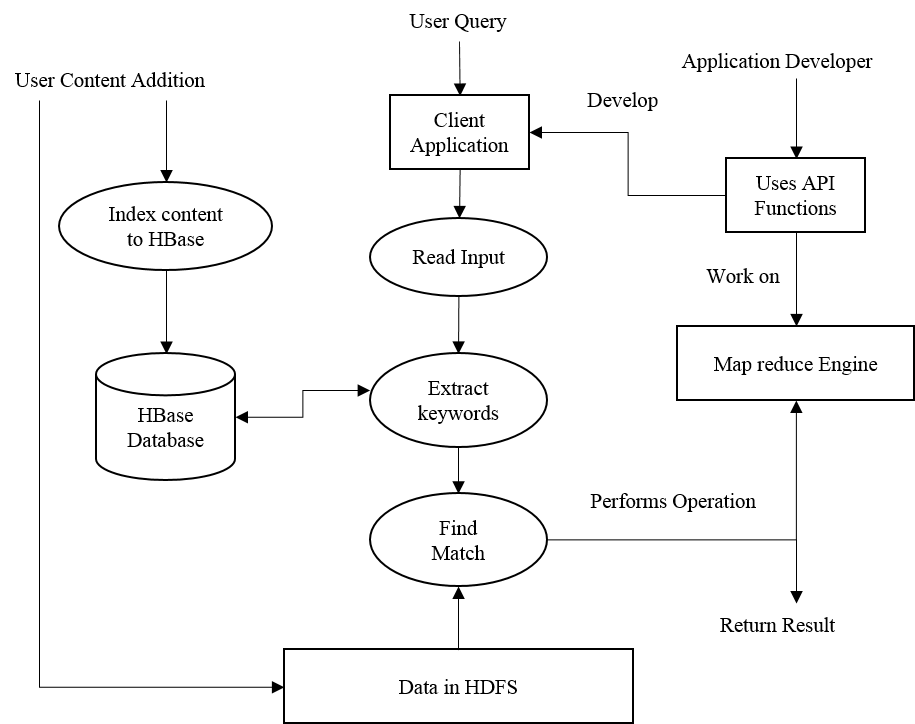
\includegraphics[width=230pt]{data_flow}}
	  \caption{Data Flow Diagram}
	  \label{fig:state-dig}
	\end{figure}
\end{center} 


\noindent \textbf{ Testing of project problem statement using generated test data (using mathematical models, GUI, Function testing principles, if any) selection and appropriate use of testing tools, testing of UML diagram’s reliability }

\section{Mathematical Model}
\noindent
S = \{s,e,x,y,DD,NDD,Mem-shared\} \\ \\
s= start state $->$ Taking input from the user as search query\\ \\ e= End State $->$ return the output to the user in the form text based content \\ \\
x = Input $->$ Search Query \\
y = Output $->$ Text Based Result \\ \\ 
DD = Deterministic Data \\
1) Number of PDF Files \\ 
2) Keyword Tokenisation and Filteration \\
3) Number of DataNodes \\
4) Search Progress \\
5) Number of Results Obtained \\ \\
NDD = Non Deterministic Data \\
1) Failure of Cluster Nodes \\
2) Communication Failure  \\ \\
Mem-Shared = Storage Space \\ 
1) HDFS will be distributed among a number of nodes in Hadoop Cluster and will share common FileSystem which will be managed by Hadoop \\

\section{Scenarios to be Tested}

\begin{center}
	\begin{figure}[H]
		\centering
		\fbox{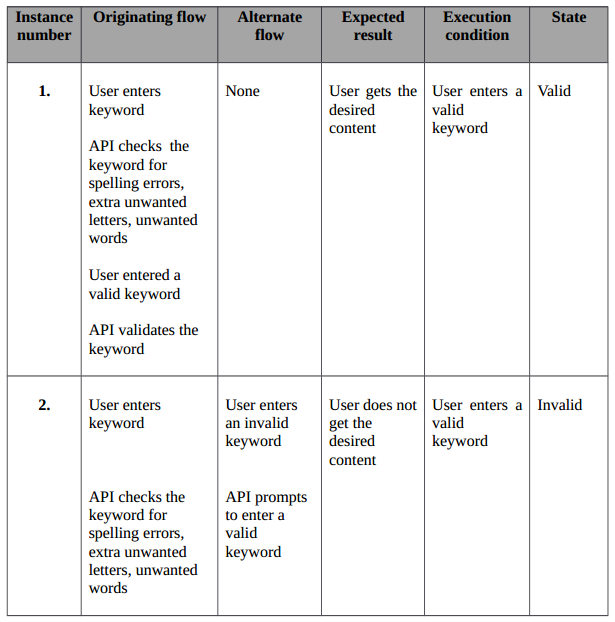
\includegraphics[width=230pt]{test-case-1}}
	  \caption{Test Case}
	  \label{fig:state-dig}
	\end{figure}
\end{center} 

\begin{center}
	\begin{figure}[H]
		\centering
		\fbox{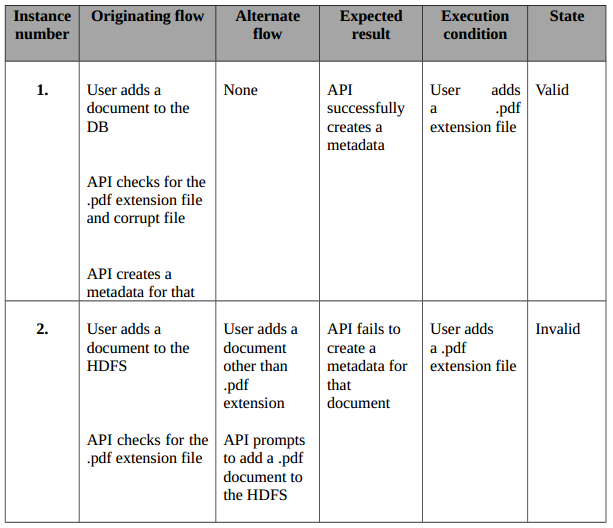
\includegraphics[width=230pt]{test-case-2}}
	  \caption{Test Case}
	  \label{fig:state-dig}
	\end{figure}
\end{center}

\begin{center}
	\begin{figure}[H]
		\centering
		\fbox{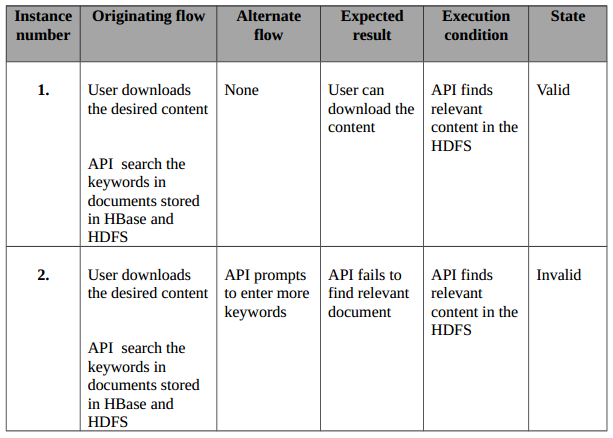
\includegraphics[width=230pt]{test-case-3}}
	  \caption{Test Case}
	  \label{fig:state-dig}
	\end{figure}
\end{center}


\chapter{Project Planner}
\label{app:plan}

Major Tasks in the Project stages are: 
\begin{itemize}
\item Create distributed system with Hadoop namenodes and datanodes
\item Develop API methods for extracting keywords from input query
\item Test API methods for finding keywords from input query
\item Develop API methods to perform keyword search on HDFS data using Map Reduce operations
\item Test API methods to perform keyword search on HDFS data using Map Reduce operations
\item Design database schema for indexing each and every document in HDFS
\item Schema validation for HBase indexing database
\item Develop background service for indexing newly added data to HBase database automatically
\item Test background service for indexing newly added data to HBase database is working automatically or not
\item Integrating all modules
\item Integration testing
\end{itemize}

\begin{center}
	\begin{figure}[!htbp]
		\centering
		\fbox{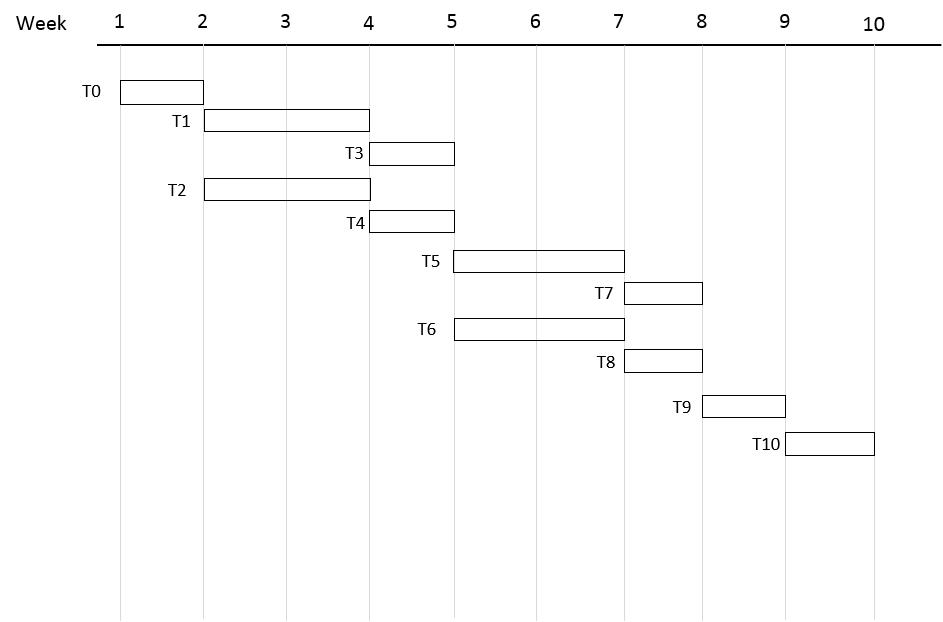
\includegraphics[width=\textwidth]{timeline_chart}}
	  \caption{Planning Chart}
	  \label{fig:usecase}
	\end{figure}
\end{center}  




\chapter{Reviewers Comments of Paper Submitted}
\begin{enumerate}
\item Paper Title: Hadoop add-on API for Advanced Content Based Search \& Retrieval
\item Name of the Conference/Journal where paper submitted : IFERP - International Conference Institute for Engineering Research and Publication
\item Paper accepted/rejected : Accepted
\item Review comments by reviewer : The reviewers committee of NIER congratulate  you for acceptance of your research paper for International Conference. You are cordially invited to convene the event by presenting your research paper through PowerPoint presentation.The Conference is being organized by NIER-India in association with "Technoarete" 

\end{enumerate}

\chapter{Plagiarism Report}
\begin{center}
	\begin{figure}[!htbp]
		\centering
		\fbox{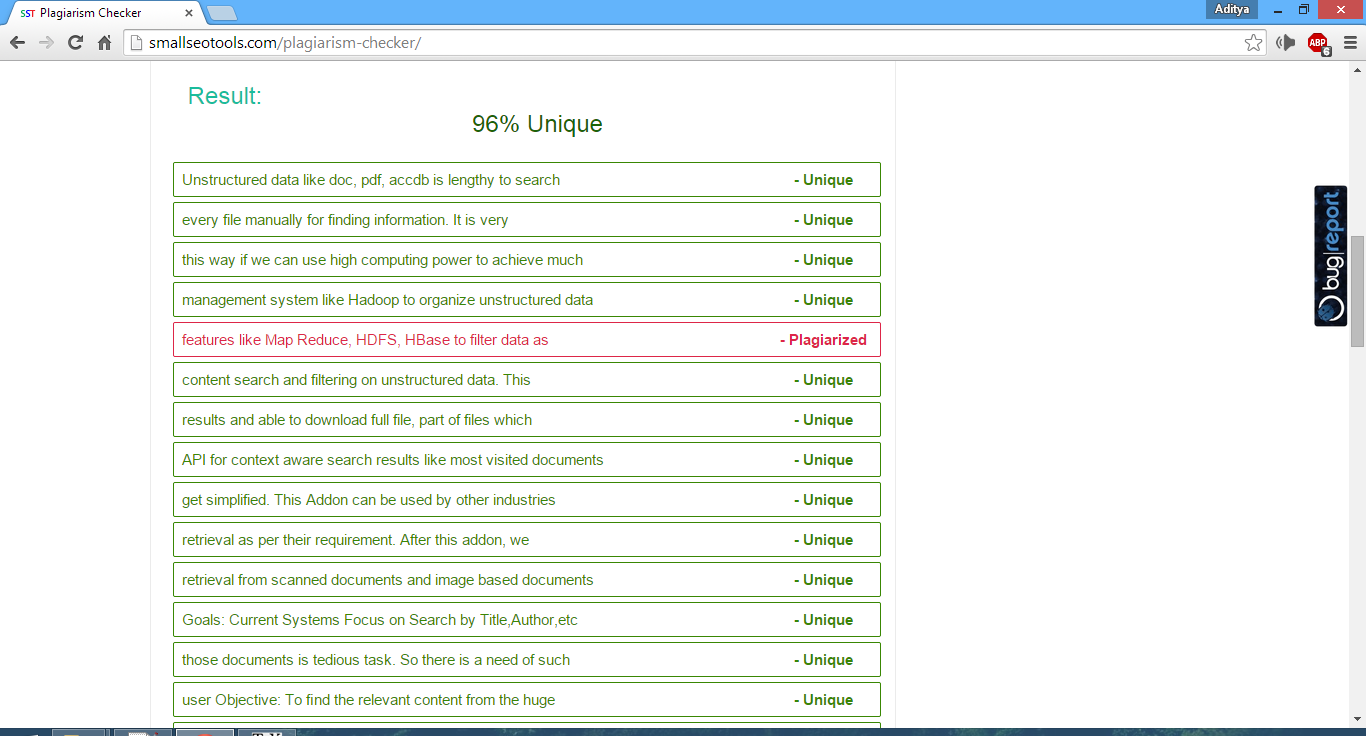
\includegraphics[width=\textwidth]{plagiarism_report}}
	  \caption{Plagiarism Report}
	  \label{fig:usecase}
	\end{figure}
\end{center}  


\end{appendices}


\end{document}
